\documentclass[]{foi} 
% zakomentirati za pisanje rada na engleskom jeziku
% comment the above line if writing in English

% \documentclass[english]{foi} 
% odkomentirati za pisanje rada na engleskom jeziku
% uncomment the above line if writing in English

\usepackage[utf8]{inputenc}


\vrstaRada{\projekt}
% \zavrsni ili \diplomski ili \seminar ili \projekt
% type of the paper:
% \seminar is a seminar/term paper
% \projekt is a project

\title{Implementacija sustava za upravljanje digitalnim certifikatima}
\predmet{Sigurnost interneta}
% ostaviti prazno ako \vrstaRada nije \projekt ili \seminar
% \predmetBP ili \predmetDP ili \predmetTBP ili \predmetVAS ili \predmetUUI
% leave it empty if \vrstaRada is not a \projekt or \seminar
% \predmetBP - Databases 1
% \predmetVAS - Multiagent Systems

\author{Denis Kuzminski \newline Karlo Jačmenjak \newline Josip Mojzeš} 
% ime i prezime studenta/studentice
% name and surname of the author
\spolStudenta{\musko} 
% \zensko ili \musko
% student's gender for grammar purposes: \zensko = F or \musko = M

\mentor{Bogdan Okreša Đurić}
% ime i prezime mentora
% name and surname of the mentor
\spolMentora{\musko} 
% \zensko ili \musko
% mentor's gender: \zensko = F or \musko = M
\titulaProfesora{doc.~dr.~sc.}
% HR: dr. sc.  / doc. dr. sc. / izv. prof. dr. sc. / prof. dr. sc. 
% mentor's title:
% EN: -prazno- / Asst. Prof.  / Assoc. Prof.       / Full Prof.

\godina{2025}
\mjesec{travanj}
% mjesec obrane rada ili projekta
% year and month of the presentation of the project or paper

\indeks{}
% broj indeksa ili JMBAG
% author's ID

\smjer{Informacijsko i programsko inženjerstvo}
% (ili:
%     Informacijski sustavi, 
%     Poslovni sustavi, 
%     Ekonomika poduzetništva, 
%     Primjena informacijske tehnologije u poslovanju, 
%     Informacijsko i programsko inženjerstvo, 
%     Baze podataka i baze znanja, 
%     Organizacija poslovnih sustava, 
%     Informatika u obrazovanju
% )
% study programme; please enter "Erasmus" for incoming exchange students


\sazetak{Digitalni certifikat je elektronički dokument koji služi za provjeru identiteta nekog uređaja, 
poslužitelja ili korisnika na internetu koristeći kriptografiju i infrastrukturu javnih ključeva. 
Certifikati se mogu koristiti u organizacijama da osiguraju da se samo pouzdani korisnici mogu 
povezati na njihove mreže te potvrđuju identitet web stranice na web pregledniku. 
Digitalne certifikate izdaju ovlaštene organizacije koje se nazivaju certifikacijsko tijelo (engl. Certificate Authority). 
Nadalje, u radu će se implementirati sustav za upravljanje digitalnim certifikatima koristeći vlastito certifikacijsko tijelo. 
Administrator sustava će moći izdati, revocirati i upravljati certifikatima. 
Također, pokazat će se implementacija provjere valjanost certifikata web poslužitelja u web pregledniku.}
% abstract of 100 to 300 words.

\kljucneRijeci{digitalni certifikat; X.509 certifikat; Certificate Revocation List; Public Key Infrastructure; Certificate Authority; HashiCorp Vault; HTTPS}
% keywords including 7 +/- 2 syntagms

\begin{document}

\maketitle

\tableofcontents

\makeatletter \def\@dotsep{4.5} \makeatother
\pagestyle{plain}

\chapter{Uvod}

Sigurnost komunikacija na internetu postaje sve važniji aspekt za uzeti u obzir zbog povećanja osjetljivih informacija koje su potrebne za rad u modernim informacijskim sustavima.
Digitalni certifikati imaju značajnu ulogu kod podizanja te sigurnosti, korištenjem kod HTTPS komunikacije podiže se razina sigurnosti razmjene informacija.
Implementacijom vlastitog sustava za upravljanje digitalnim certifikatima postiže se neovisnost i potpuna kontrola nad izdavanjem certifikata.
Međutim upravljanje životnim ciklusom certifikata može biti izazovno ako se radi o velikoj količini certifikata.

Kroz praktični dio rada korišten je HashiCorp Vault.
Primarno je namijenjen čuvanju tajni, ali ima mogućnost izdavanja digitalnih certifikata.
Kroz teorijski dio također je predstavljen Dogtag sustav certifikata za dugoročno i preciznije upravljanje certifikatima.

Cilj projekta je izrada sustava za upravljanje digitalnim certifikatima kod HTTPS komunikacije.
Projekt uključuje implementaciju alata za izdavanje, revociranje i upravljanje certifikatima te implementaciju protokola za provjeru valjanosti certifikata.


\chapter{Digitalni certifikati}

Digitalni certifikat predstavlja datoteku pomoću koje je omogućena autentifikacija za razne uređaje korištenjem kriptografije ili sustava javnih ključeva \cite{fortinet-digital-certificates}.
Glavna uloga digitalnih certifikata je da omoguće mrežni pristup samo pouzdanim uređajima.
Digitalni certifikat je našao veliku primjenu kod dokazivanja web stranice prema web pretraživaču.
Sadrži identifikacijske informacije te IP adresu ili serijski broj uređaja.
Digitalni certifikat također sadrži kopiju javnog ključa koji je izdan od strane izdavača certifikate te ona služi kod potvrde valjanosti certifikata.

Tijela za izdavanje certifikata (engl. certificate authorities - CA) se brinu o valjanosti postojećih te izdavanju novih digitalnih certifikata.
Digitalni certifikati su jedan od načina primjene kibernetičke sigurnosti.
Digitalni certifikati pružaju: sigurnost, skalabilnost, autentičnost, pouzdanost i javno povjerenje.
Nekada dolazi do miješanja pojmova digitalnih certifikata i digitalnih potpisa.
Digitalni potpis za razliku od certifikata osigurava integritet i autentičnost dokumenta ili e-pošte pomoću kriptografskog ključa kreiranog od vlasnika dokumenta dok certifikat potvrđuje identitet.

Povlačenje odnosno opoziv valjanosti certifikata se može provesti na više načina: online ili offline provjera, pomoću liste odobrenih i zabranjenih, pomoću vođenje evidencije i pomoću distribucije informacije.
Razlozi za opoziv mogu biti razni, a neki od najčešćih razloga su: kompromitiran ključ, promjena informacija u certifikatu, zamjena certifikata, nepotreban certifikat.
Opoziv se može provesti i zbog drugih razloga poput probijanja algoritma šifriranja, a svaki taj razlog se obično navodi kao informacija uz certifikat koji je opozvan.
Postoje liste opoziva certifikata odnosno CRL (engl. certificate revocation lists) koje sadrže ključne informacije o opozivanim certifikatima.
Ovakve liste pružaju laku provjeru valjanosti, ali može biti problem njihova veličina jer je današnji broj digitalnih certifikata velik.
Liste se nalaze u sustavu za opoziv certifikata odnosno CRS (engl. certificate revocation system) koji sadrže evidenciju pozitivnih i negativnih lista.
Kako bi liste bile ažurirane i točne tijela za izdavanje certifikata šalju najnovije informacije o certifikatima.[12]

\chapter{Kriptografija}

Kriptografija je sposobnost korištenja algoritama za zaštitu poruka od neovlaštenog čitanja \cite{ibm-cryptography}.
Poruka koja se prenosi od kreatora poruke prema primatelju za treću stranu mora biti nerazumljiva.
Ovakva nečitljiva poruka (engl. ciphertext) se može pročitati jedino korištenjem ključa te algoritma koji se koristio tijekom kriptiranja, a izlaz je čitljiv tekst (engl. plain text).
Kriptografija u današnje doba osigurava 4 osnovna principa: integritet, neporecivost, povjerljivost i autentifikaciju.
Kriptografija i kriptografski algoritmi osiguravaju svu sigurnost i privatnost informacija koje se koriste kroz informatičke sustave.
Osnovna područja u kojem se primjenjuje: upravljanje lozinkama, kriptovalute, sigurno web pretraživanje, elektronički potpis, autentifikacija te sigurna komunikacija.
Postoje dvije osnovne vrste kriptografije, a to su: simetrična i asimetrična kriptografija.

\section{Simetrična kriptografija}

Simetrična kriptografija koristi jedan ključ za enkripciju i dekripciju, a to znači da pošiljatelj i primatelj imaju jednak ključ kod sebe. Simetrična kriptografija je brza, efikasna te osigurava povjerljivost, no problem može biti čuvanje ključa kojim se radi enkripcija i dekripcija. Najveću primjenu pronalazi kod šifriranja velike količine podataka.


\section{Asimetrična kriptografija}

Za razliku od simetrične, asimetrična kriptografija koristi dva ključa privatni i javni.
Poruka se kriptira na način da se koristi privatni ključ pošiljatelja te javni ključ, a dekriptira se korištenjem privatnim ključem primatelja te javnim ključem.
Ovakav način kriptiranja/dekriptiranja osigurava da privatnom ključu (koji je jedan od dva potrebna dijela) imaju pristup samo vlasnici ključa.
Isto tako javni ključ se može dijeliti preko nesigurnih kanala komunikacije što olakšava primjenu.
Asimetrična kriptografija pruža sigurnost i robusnost, ali zahtjeva puno više resursa i vremena od simetrične kriptografije.
U modernim kriptografskim sustavima često se koristi kombinacija simetričnih i asimetričnih algoritama kako bi se iskoristile prednosti oba pristupa. Simetrični ključ, koji se koristi za šifriranje podataka, najprije se enkriptira pomoću asimetričnog algoritma i sigurno se prenosi primatelju. Nakon toga, primatelj dešifrira simetrični ključ pomoću svog privatnog ključa i koristi ga za daljnju komunikaciju.

\noindent Primjeri sustava koji koriste ovu metodu su:
\begin{itemize}[noitemsep,topsep=0pt]
    \item TLS (Transport Layer Security) - koristi RSA ili ECC za razmjenu ključeva i AES za šifriranje podataka.
    \item PGP (Pretty Good Privacy) - koristi RSA za šifriranje sesijskog ključa, dok se stvarna enkripcija podataka vrši simetričnim algoritmom poput AES-a.
    \item Signal protokol - koristi kombinaciju asimetrične kriptografije (Double Ratchet algoritam) i simetrične enkripcije za sigurno slanje poruka.
\end{itemize}


\chapter{Infrastruktura javnih ključeva}

PKI (engl. public key infrastructure) odnosno infrastruktura javnih ključeva upravlja izdavanjem digitalnih certifikata
\cite{keyfactor-pki}.
Sve velike organizacije kojima je stalo do sigurnosti koriste indirektno ili direktno PKI jer se on brine o valjanosti i sigurnosti ključeva potrebnih za enkripciju.
PKI rješava izazove oko potvrde vlasnika ključa da je pošiljatelj neke poruke zaista onaj za kojeg se predstavlja.
Digitalni certifikati se često nazivaju PKI certifikati ili X.509 certifikati.
PKI se prvi puta pojavljuje 1990-ih te se slabo primjenjuje jer je izrada certifikata skupa i dugo traje.
Digitalne certifikate su koristile tvrtke koje su npr. imale online trgovine i željele pružiti sigurnost prilikom kupovine.
Prva veća potreba za PKI-om desila se 2000-ih pojavom udaljenog rada (van ureda).
Zaposlenici se spajaju preko VPN-a (engl. virtual private network) odnosno virtualne privatne mreže na mrežu tvrtke.
Kako bi tvrtka bila posve sigurna u identitet osobe koja se spaja na njegovu mrežu ugrađuje digitalne certifikate na računala zaposlenika.
Neki od njih kupuje certifikate, a neki implementiraju vlastite.
Velika količina certifikata zahtjeva dobro upravljanje njima kako ne bi istekli ili bili kompromitirani.
Od 2010-ih do danas potreba za PKI-em i digitalnim certifikatima sve je veća.
Jedan od uzroka sve veće potrebe je pojava miliona uređaja IoT (engl. internet of things) odnosno internet stvari.
Takvi uređaji zahtijevaju spajanje na mrežu, a veza mora biti sigurna.
Upravljanje velikom količinom certifikata postaje sve napornije i tvrtke se često odlučuju na angažiranje pružatelje usluge za PKI.

Neki od najčešće korištenih slučajeva PKI-a su: SSL/TLS certifikati za sigurno pretraživanje, digitalni potpis na softveru, upravljan pristup mreži te e-mail i podatkovna enkripcija.
IoT uređaji su ranjivi zato jer često imaju jednostavna softverska rješenja koja su manje izazovna za hakere.
Kako bi se takvi uređaji zaštitili potrebno je ugraditi certifikate koji omogućuju sigurnu komunikaciju.
Primjeri IoT uređaja koji moraju biti maksimalno sigurni su u auto industriji i medicinskoj industriji.
Svaki napredni uređaj koji ima više točaka povezivanja na neku vrstu mreže može predstavljati opasnost od zlonamjernog korištenja.
Zlonamjerno korištenje uređaja koji su ugrađeni u automobile ili medicinsku opremu mogu dovesti do katastrofalnih posljedica poput gubitka ljudskih života.
Kako bi se veze prema takvim uređajima zaštitile PKI izdaje certifikate uređajima te softveru s kojima uređaji komuniciraju.
Uvođenje PKI može biti izazovno no sigurnost koju donosi korištenje digitalnih certifikata je najvažnija.

\pagebreak

\section{Dogtag Certificate System}

Dogtag sustav certifikata (engl. certificate system) \cite{dogtagpki} je tijelo za izdavanje certifikata otvorenog koda.
Ovaj sustav je kompletan odnosno omogućuje upravljanje cijelim životnim ciklusom certifikata.
Sustav je besplatan za korištenje te donekle jednostavan za implementaciju.
Dogtag je skup tehnologija, a neke od ključnih značajki sustava su:

\begin{itemize}[noitemsep,topsep=0pt]
    \item izdavanje, opoziv i pronalaženje certifikata,
    \item generiranje i objavljivanje popisa opozvanih certifikata (CLR),
    \item jednostavni upis certifikata (SCEP),
    \item arhiviranje i omogućen oporavak ključa za šifriranje,
    \item upravljanje životnim ciklusom pametne kartice,
    \item opsežna dokumentacija te snažna zajednica korisnika.
\end{itemize}


\subsection{Arhitektura}

Dogtag PKI sustav certifikata pokreće se kao web aplikacija na Tomcat serveru \cite{dogtagpki-architecture}.
Ovakva struktura omogućuje korisnicima i klijentskim aplikacijama pristup putem različitih sučelja.
Zajednički okvir napisan u Javi osigurava upravljanje, bilježenje, autentifikaciju, kontrolu pristupa, samotestiranje i kreiranje obavijesti.
Kao bazu podataka sustav koristi 389 Directory Server za pohranu svih ključnih informacija.
Sustav s internom LDAP bazom komunicira na siguran način pomoću SSL protokola.
\subsection{NSS}
NSS (engl. network security services) odnosno usluge mrežne sigurnosti su skup biblioteka koje omogućuju više platformni razvoj aplikacija sa sigurnosni omogućenom komunikacijom.
Aplikacije napravljene na ovakav način omogućuju korištenje SSL protokola za autentifikaciju, otkrivanje neovlaštenih izmjena i šifriranja te PKCS\#11 za sučelje kriptografskih tokena.
Red Hat koristi NSS u širokom spektru proizvoda, uključujući sustav certifikata.
\subsection{Standardno PKCS\#11 sučelje}
PKCS\#11 (engl. public-key cryptography standard) je standard koji specificira API koji se koristi za komunikaciju sa uređajima koji sadrže kriptografske informacije i izvode kriptografske operacije.
Na ovakav način omogućeno je korištenje na različitom softveru i hardveru.
\subsection{JSS i sloj JNI}
JSS (engl. network security services for Java) pruža sučelje za sigurnosne operacije koje izvodi NSS.
JSS je izrađen s JNI (engl. Java native interface) koji omogućava binarnu kompatibilnost između različitih JVM-a (engl. Java virtual machine).
Ovakav dizajn omogućuje izradu jednom, a pokretanje više puta na različitim platformama.
\pagebreak
\section{HashiCorp Vault}

HashiCorp Vault je temeljen na sigurnosti identiteta i sustav je koji upravlja enkripcijom \cite{hashicorp-vault-what-is}.
Obavlja usluge enkripcije koje su osigurane autentifikacijom i autorizacijskim metodama kako bi se osigurala sigurnost, onemogućen pristup trećim stranama te praćenje izvršenih radnji.
Vault pruža sučelje za bilo koju vrstu tajne poput tokena, zaporke, API ključa itd. osiguravajući strogu kontrolu pristupa te bilježenje izvršenih radnji.
Vault provjerava klijente odnosno korisnike koji žele pristupit tajnama te im sukladno dodijeljenim pravima omogućuje pristup.

\subsection{Kako radi Vault?}

Vault primarno radi s tokenima koji su povezani s putanjama prema servisu, a token ordređuje koje radnje i prava pristupa klijent posjeduje.

\begin{figure}[htbp]
    \centering
    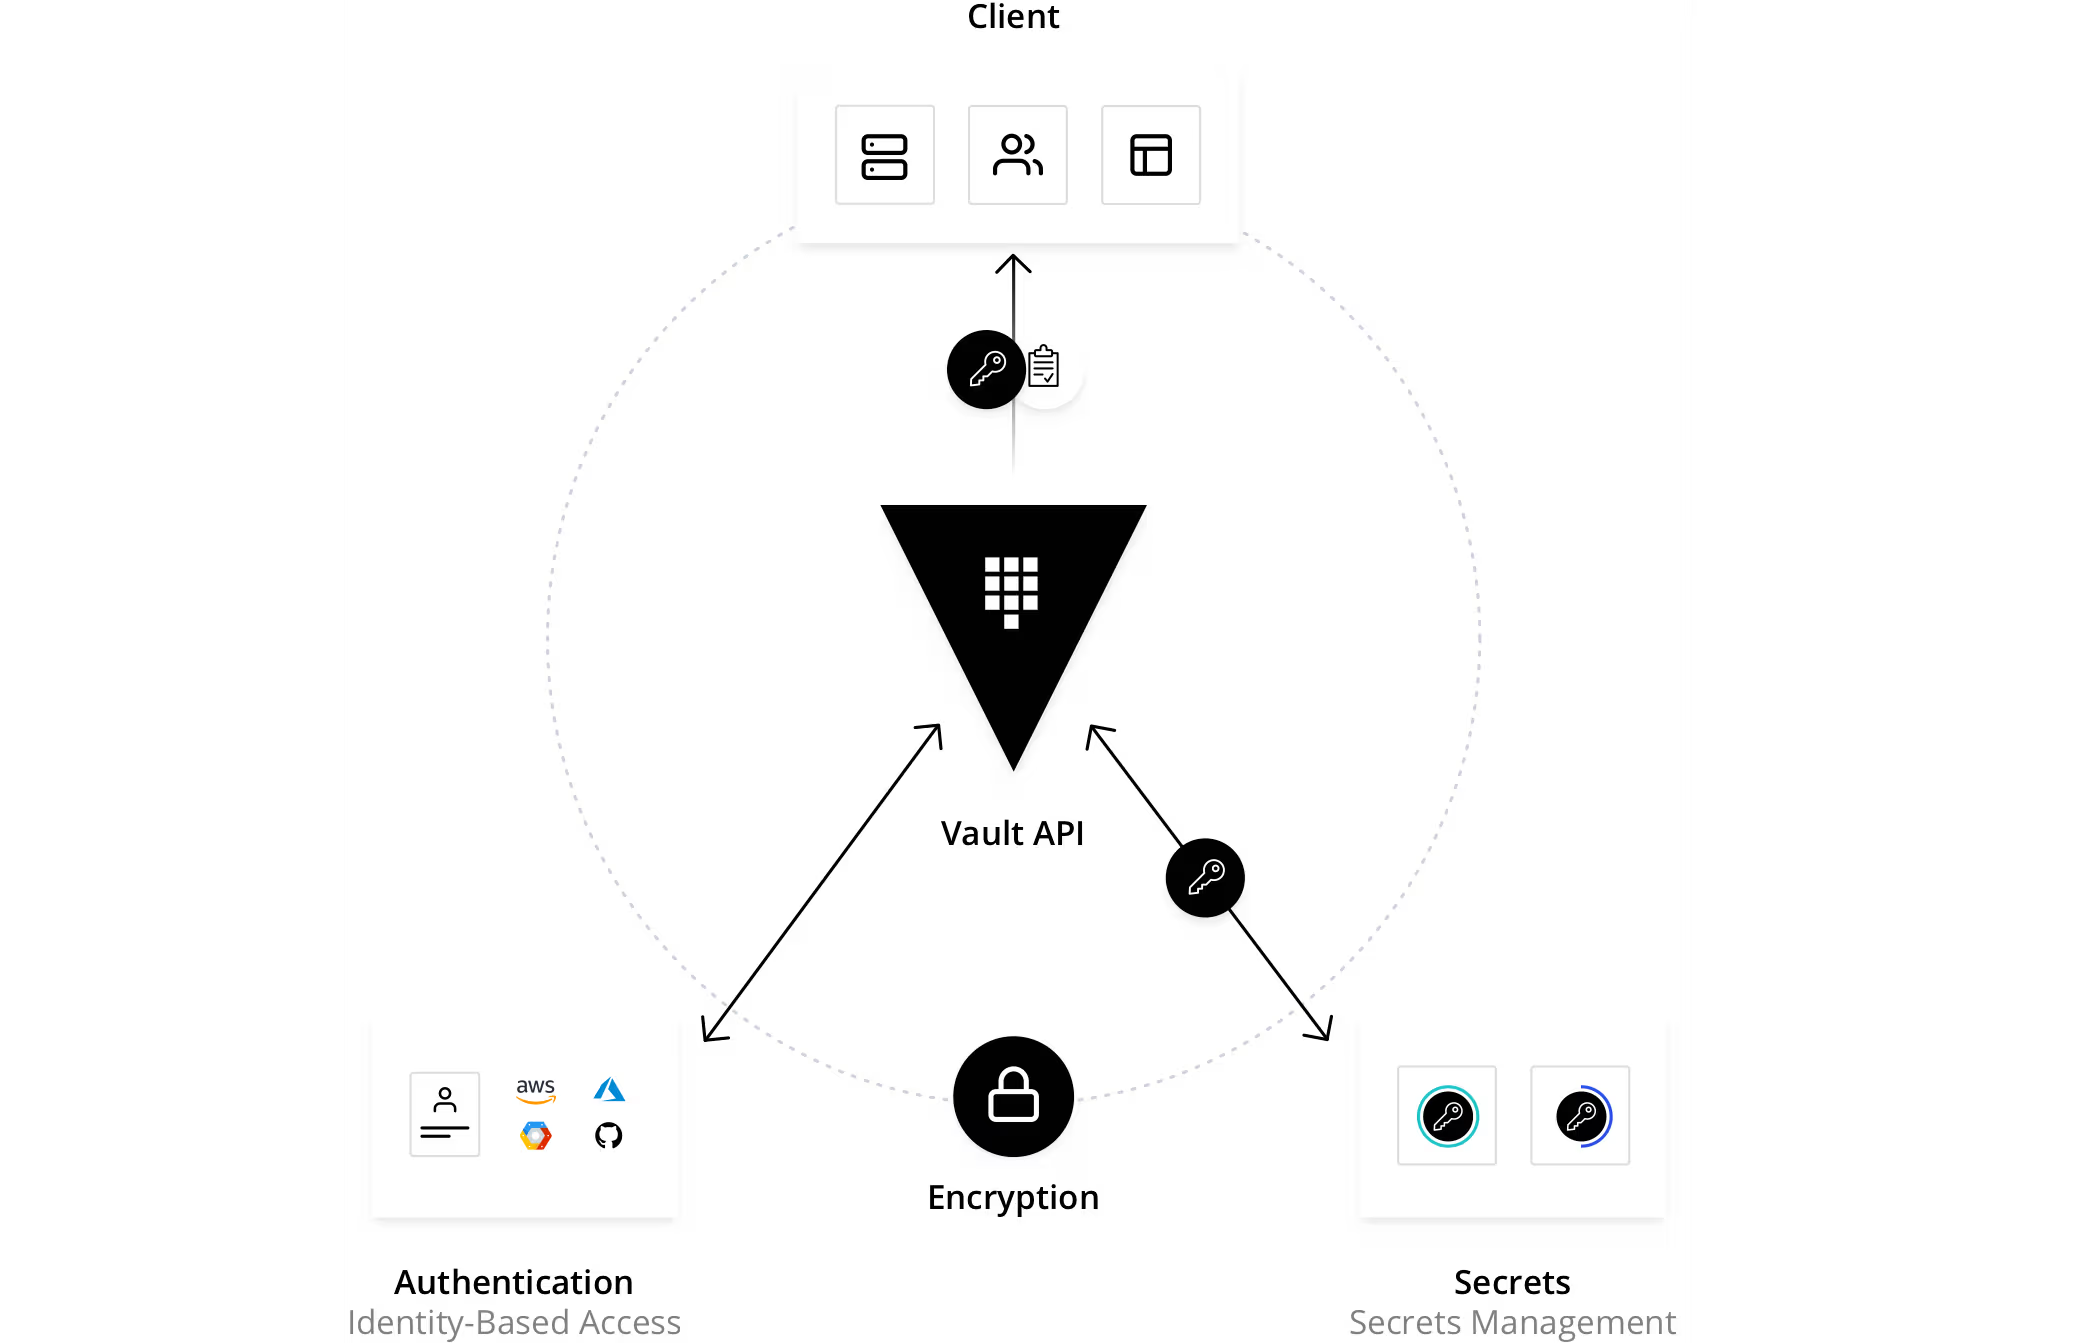
\includegraphics[width=1.0\textwidth]{assets/hashicorp-arhitektura.png}
    \caption{HashiCorp Vault Arhitektura \cite{hashicorp-vault-what-is}}
\end{figure}

Slika prikazuje na koji način Vault radi.
Cijeli proces započinje autentifikacijom, zatim Vault provjerava identitet klijenta uz pomoć neke pouzdane treće strane.
Slijed proces autorizacije i usklađivanja prava na strani klijenta na način da mu se dopušta pristup tajnim informacijama prema unaprijed definiranim pravilima.

\pagebreak

\subsection{Značajke Vault-a}

Vault je dizajniran na način da centralizira i s jednog mjesta upravlja svim vjerodajnicama koje bi inaće neka tvrtka držala na više potencijalno nesigurnih mjesta.
Vault osigurava da su svi korisnici, aplikacije i sustavi prošli autentifikaciju te da su autorizirani za pristup vjerodajnicama.
Također osigurava da je snimljena sva povijest radnji klijenta.
Kako bi se zaštitile informacije Vault ih prije spremanja enkriptira te takve sprema u pohranu, na ovaj način podiže se sigurnost pohrane informacije.
Omogućuje dinamičko dodjeljivanje pristupa nekim tajnim informacijama, može po potrebi dati pristup nekoj tajni te nakon nekog vremena povući to pravo pristupa.
Omogućuje enkripciju i dekripciju podataka koje prenosi bez spremanja u neku pohranu.
Vault ima ugrađeni sustav povlačenja tajni, ako se desi neki upad u sustav na ovaj način se može zaključati sustav te spriječiti uništenje sustava.

\subsection{HashiCorp Cloud Platform}

Postoji inačica Vaulta koju HashiCorp nudi kao uslugu odnosno koja je instalirana na nekom udaljenom poslužitelju.
Ova inačica pruža brži i jednostavniji pristup, a korištenje odnosno komunikacija prema Vaultu ostaje ista kao i kod samostalne implementacije.
Takav pristup omogućuje smanjenje operativnih troškova te uklanja brige oko nadogradnji i sigurnosnih kopija.
Jednostavnost, pouzdanost i lakša kontrola kod ovakvog pristupa omogućuje organizaciji ili tvrtki veći fokus na ostale poslove.


\subsection{Korištenje Vault-a}

Kao što je i prethodno navedeno Vault se bavi upravljanjem osjetljivim i tajnim informacijama koje organizacija posjeduje.
U nastavku će se obraditi na koje načine se koristi Vault.

Posjedovanje vjerodajnica s dugim rokom za organizaciju predstavlja prijetnju.
Vault omogućuje stvaranje i upravljanje vjerodajnicama koje će biti korištene kratko ili s nekim vremenskim ograničenjem uz automatsko povlačenje ili mijenjanje prava koje donosi vjerodajnica.
Vjerodajnica mogu biti dugovječne i statičke te se kao takve čuvaju zaštićene i spremljene te se koriste samo na zahtjev klijenta.
Isto tako vjerodajnice mogu biti dinamičke odnosno one nastaju kada klijent ima potrebu za njima.
Vault može upravljati vremenskim ograničenjima te brisanjem samih vjerodajnica nakon isteka nekog roka.

Vault nudi uslugu enkripcije kao usluge kako se organizacija ne bi morala zamarati s održavanjem ključeva i samom kriptografijom.
Vault može enkriptirati ili dekriptirati podatke pohranjene bilo gdje te se u potpunosti brine da su podaci zaštićeni.

Vault također nudi uslugu upravljanja pristupom na temelju identiteta korisnika.
Koristi se ACL sustav koji povezuje identitet među različitim pružateljima usluga te kao posrednik brine o pristupu sustavima i tajnama. Vault nudi svoj sustav za upravljanje ključevima koji brine o distribuciji i životnom ciklusu ključeva, a korisnicima usluge omogućuje centralizirani pristup i standardne kriptografske mogućnosti koji omogućavaju drugi pružatelji usluge upravljanja ključevima. \cite{hashicorp-vault-use-cases}

\subsection{Certifikacijsko tijelo u HashiCorp Vault-u}

Vault PKI može dinamički izraditi X.509 certifikat na zahtjev, a izrada certifikata je brza i sigurna. \cite{hashicorp-vault-pki-engine} Vault PKI engine implementira funkcionalnost vlastitog certifikacijskog tijela unutar Vault sustava. Uloga ovog modula je dinamičko izdavanje X.509 certifikata prema unaprijed definiranim pravilima i postavkama. Ključne značajke ovog pristupa uključuju:

\begin{itemize}
    \item \textbf{Dinamičko izdavanje certifikata} - Certifikati se mogu generirati na zahtjev (bilo to pomoću nekog sučelja ili programski preko REST API-ija), čime se eliminira potreba za dugotrajnim, statičkim certifikatima i smanjuje rizik od njihovog kompromitiranja.
    \item \textbf{Definiranje uloga} - Administratori mogu kreirati uloge koje specificiraju uvjete poput trajanja certifikata, dozvoljenih domena te drugih parametara, čime se omogućuje fleksibilno i kontrolirano izdavanje certifikata.
    \item \textbf{Automatizacija i sigurnost} - Proces izdavanja i revokacije certifikata je automatiziran, što smanjuje mogućnost ljudskih pogrešaka te osigurava visoku razinu sigurnosti kroz strogu kontrolu pristupa i bilježenje svih operacija.
\end{itemize}

Uz to Certifikacijsko tijelo unutar Vault-a dopušta kreiranje korijenskih certifikata (\textit{root certificates}), srednjih certifikata(\textit{engl. intermediate certificate}) i idetifikacijskih (poslužiteljskih) certifikata (\textit{indentity certificate}). Srednji certifikati se granaju od korijenskih certifikata poput grana drveća. Oni djeluju kao posrednici između zaštićenih korijenskih certifikata i poslužiteljskih certifikata koji se izdaju javnosti. U lancu će uvijek postojati barem jedan posredni certifikat, ali može ih biti i više. poslužiteljski certifikati služe za izdavanje krajnjim korisnicima neke domene za koju certifikacijsko tijelo izdaje certifikate. Oni omogućavaju kreiranje pod-domena (\textit{engl. subdomains}) za danu domenu. Na slici ispod prikazana je pod-domena \textit{test.example.com} za domenu \textit{example.com} koja štiti korijenski certifikat.

\begin{figure}[htbp]
    \centering
    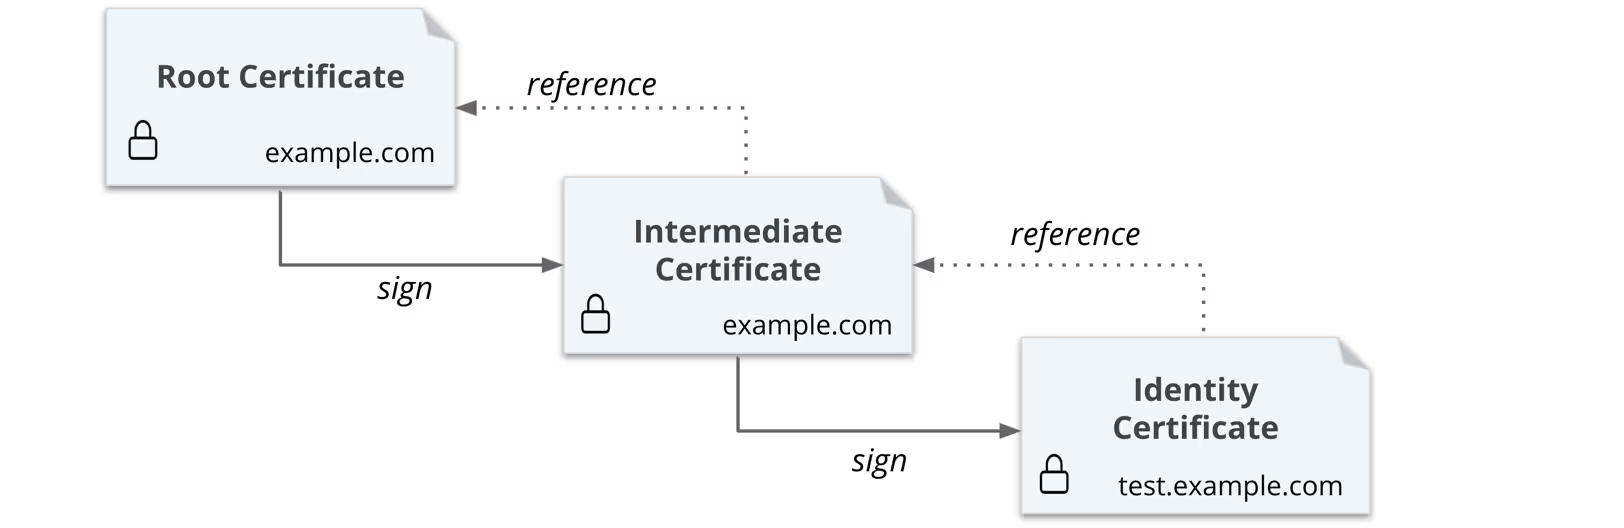
\includegraphics[width=1.0\textwidth]{assets/hashicorp-certificates.png}
    \caption{Prikaz samo-potpisujućeg korijenskog certifikata i srednjih certifikati \cite{hashicorp-vault-pki-engine}}
\end{figure}


\chapter{X.509 certifikat}

X.509 certifikat je digitalni certifikat koji se temelji na X.509 PKI standardu kojim se provjerava identitet nekog korisnika ili sustava.
PKI omogućuje sigurnu komunikaciju između korisnika i nekog servisa.
X.509 certifikat je definiran od strane International Telecommunication Union's Telecommunication Standardization Sector (ITU-T), a trenutna verzija 9 je definirana u listopadu 2019. godine.
Verzijama se zapravo definira šta sve sadrži te na koji način certifikat sprema informacije.
Certifikat X.509 sadrži informacije: o verziji, serijskom broju, algoritmu koji se koristio tijekom potpisa, imenu izdavatelja, trajanju certifikata, imenu korisnika, informacije o javnom ključu i opcionalno neko proširenje.
\cite{techtarget-x509-certificate}

\section{Primjena X.509 certifikata}

Primjena X.509 certifikata koji sadrži javni ključ i identitet je široka te se koristi kada je potrebna sigurnost u komunikaciji ili kao dokaz vjerodostojnosti.
Do certifikata se dolazi na način da korisnik pošalje zahtjev za izdavanje certifikata, web server proslijedi zahtjev prema CA te CA izda certifikat.
Izrađen X.509 certifikat se može koristi kod digitalnih identiteta, TLS/SSL, sigurnog web pretraživanja, digitalnih potpisa, SSH, e-mail certifikata i sl.
Može se primijetiti da mu je primjena široka, a pruža zaštitu od potencijalnih prijetnji koje nastaju od zlonamjernih trećih strana koje se lažno predstavljaju.
\cite{techtarget-x509-certificate}

\chapter{HTTP i HTTPS}

HTTP (engl. hypertext transfer protocol) je protokol aplikacijskog sloja koji prikazuje podatke na web mjestu razumljive ljudima.
HTTP sa serverom koji sadrži informacije komunicira preko HTTP zahtjeva i porta 80.
HTTP zahtjevi koje postavlja prema serveru su: CONNECT, GET, POST, PUT, DELETE, HEAD, OPTIONS.
Uobičajen HTTP zahtjev sadrži: HTTP verziju, URL, HTTP metodu, HTTP zaglavlje zahtjeva i opcionalno HTTP tijelo.
Server prema klijentu odgovara pomoću HTTP odgovora koji sadrži: HTTP kod statusa, HTTP zaglavlje odgovora i opcionalno HTTP tijelo.
Najpoznatiji je HTTP kod statusa koji se sastoji od 3 znamenke, a označavaju status odgovora na zahtjev poslan prema serveru.
Općenito prvi broj u kodu statusa označuje grupu kojoj kod pripada, to su: 1xx informacija, 2xx uspjeh, 3xx preusmjeravanje, 4xx error klijenta, 5xx error servera.
\cite{cloudflare-http}

HTTPS (engl. hypertext transfer protocol secure) je sigurna verzija HTTP-a odnosno koristi kriptirani promet prilikom prijenosa informacija.
Bilo koja web stranica ili aplikacija koja isporučuje ili prima osjetljive informacije trebala bi imati ugrađen HTTPS protokol.
Bez ugrađenog HTTPS protokola najjednostavnijim snimanjem prometa koji se dešava između klijenta i servera može se doći do svih informacijama u čistom tekstu.
Kako bi se spriječilo takvo neometano čitanje HTTPS koristi protokol TLS (engl. transport layer security) ili takozvani SSL (engl. secure sockets layer) koji asimetričnom kriptografijom šifrira podatke.
U ovom slučaju ako dođe do snimanja prometa on je nerazumljiv i nečitljiv.
HTTPS za komunikaciju koristi port 443, a zahtjevi su isti kao i kod HTTP-a.
Za razliku od HTTP-a, HTTPS prije komunikacije s nekim servisom koristi TLS/SSL rukovanje (engl. handshake) kod kojeg se koristi TLS/SSL certifikat za potvrdu identiteta.
\cite{cloudflare-https}

\chapter{Implementacija sustava}

Sustav za upravljanje digitalnim certifikatima biti će izrađen kao web aplikacija koja će u pozadini koristiti HashiCorp Vault \cite{hashicorp-vault-what-is}.
Također, koristeći HashiCorp Vault, napravit će se vlastito certifikacijsko tijelo za izdavanje digitalnih certifikata.

Web aplikacija za upravljanje certifikatima će administratoru sustava omogućiti sljedeće funkcionalnosti:
\begin{itemize}
    \item \textbf{Autentifikacija} - Administrator će se morati autentificirati kako bi mogao koristiti sustav.
    \item \textbf{Prikaz i upravljanje ulogama} - Administrator će moći pregledavati, dodavati, uređivati i brisati uloge.
          Uloga označava predložak prema kojem se potpisuju digitalni certifikati korisnika.
    \item \textbf{Prikaz certifikata} - Administrator će moći vidjeti sve certifikate koje je izdalo vlastito certifikacijsko tijelo.
          Za svaki certifikat, administrator će vidjeti identifikacijske podatke o subjektu te razdoblje za koje je izdan certifikat.
    \item \textbf{Izdavanje certifikata} - Administrator će moći izdati, odnosno potpisati digitalni certifikat korisnika.
          Administrator će izdati certifikat na temelju zahtjeva za potpisivanje certifikata (engl. Certificate signing request) kojeg će generirati korisnik za kojeg se izdaje certifikat.
    \item \textbf{Revociranje certifikata} - Administrator će moći revocirati certifikat, odnosno proglasiti ga nevažećim.
\end{itemize}

Nadalje, napravit će se jednostavan HTTPS poslužitelj kojim će se prikazati način provjere valjanosti digitalnog certifikata u web pregledniku.
HTTPS poslužitelj će posluživati jednostavnu web stranicu te će u ovom dijelu biti objašnjeno kako napraviti HTTPS poslužitelj koji će koristiti
vlastiti certifikat koji je potpisan od vlastitog certifikacijskog tijela.

\pagebreak

U nastavku je prikazana arhitektura sustava za upravljanje digitalnim certifikatima.

\begin{figure}[htbp]
    \centering
    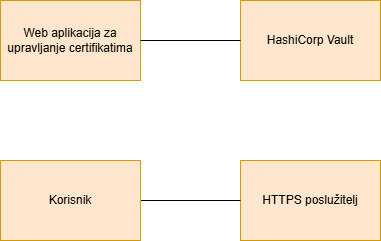
\includegraphics[width=0.8\textwidth]{assets/arhitektura.png}
    \caption{Prikaz arhitekture sustava za upravljanje digitalnim certifikatima}
\end{figure}

Sustav se sastoji od 4 dijela:
\begin{itemize}
    \item \textbf{Web aplikacija za upravljanje certifikatima} - Web aplikacija komunicira s HashiCorp Vault backend-om te omogućuje administratoru upravljanje digitalnim certifikatima.
    \item \textbf{HashiCorp Vault} - HashiCorp Vault omogućuje pokretanje vlastitog certifikacijskog tijela,
          poslužuje REST API za upravljanje certifikatima i sigurno ih pohranjuje.
    \item \textbf{HTTPS poslužitelj} - HTTPS poslužitelj poslužuje jednostavnu web stranicu, a cilj mu je prikazati način postavljanja
          HTTPS poslužitelja.
    \item \textbf{Korisnik} - Korisnik komunicira s HTTPS poslužiteljem i provjerava valjanost digitalnog certifikata.
\end{itemize}

\chapter{Zaključak}

U ovom radu analizirana je važnost digitalnih certifikata u osiguravanju sigurnosti internetskih komunikacija.
Implementacija vlastitog sustava za upravljanje digitalnim certifikatima, uz primjenu alata kao što je HashiCorp Vault,
omogućava pouzdanu i skalabilnu infrastrukturu za provjeru identiteta te zaštitu osjetljivih podataka.
Korištene su metode i tehnike temeljene na primjeni X.509 certifikata, simetrične i asimetrične kriptografije,
što je rezultiralo efikasnijim upravljanjem životnim ciklusom certifikata i smanjenjem rizika od kompromitacije.
Proces izdavanja i opoziva certifikata dodatno doprinosi visokoj razini sigurnosti, dok su primijenjeni programski
alati omogućili fleksibilnost i prilagodbu sustava specifičnim potrebama organizacije.
Rad pokazuje da implementacija vlastitog certifikacijskog tijela predstavlja fleksibilno 
rješenje u organizacijama koje žele zaštititi svoje sustave.

\makebackmatter
% generira popis korištene literature, popis slika (ako je primjenjivo), popis tablica (ako je primjenjivo) i popis isječaka koda (ako je primjenjivo)

% \appendices % ako nije potrebno, obrisati ili zakomentirati

% \chapter{Prilog 1} % ako nije potrebno, obrisati ili zakomentirati

% \chapter{Prilog 2} % ako nije potrebno, obrisati ili zakomentirati

\end{document}
